\newpage
\section{Auswertung}

In diesem Abschnitt wird der Versuch ausgewertet.

\subsection{Berechnung der Flächenträgheitsmomente}
Zunächst müssen die Flächenträgheitsmomente der Stäbe berechnet werden. Es liegen drei Arten von Stäben vor. Zwei mit runder und jeweils einer mit rechteckiger und  
 quadratischer Querschnittsfläche.

\noindent
Für den runden Stab gilt, mit $d$ als den Durchmesser,
\begin{align}
    \symbf{I}_\text{R} &= \int_0^{2\pi} \int_0^\frac{d}{2} (r \cdot \sin(\varphi))²\cdot \symup{d}r \symup{d}\varphi
    = \frac{1}{4}\left(\frac{d}{2}\right)⁴ \int_0^{2\pi} \sin(\varphi)² \symup{d}\varphi\\
    &= \left.\frac{d⁴}{64} \frac{\varphi}{2} - \frac{\sin(\varphi) \cos{\varphi}}{2} \right|_0^2\pi
    = \frac{\pi}{64} d⁴.
    \label{eqn:Rund}
\end{align}

\noindent
Für einen Stab mit rechteckiger Querschnittsfläche folgt dann äquivalent mit den Seitenlängen $a$ und $b$
\begin{equation}
    \symbf{I}_\text{Recht} = \int_\frac{-a}{2}^\frac{a}{2} \int_\frac{-b}{2}^\frac{b}{2} y² \symup{d}y \symup{d}z 
    = \int_\frac{-b}{2}^\frac{b}{2} \frac{a³}{12} \symup{d}z 
    = b \cdot \frac{a³}{12} 
    = \frac{a⁴}{12}
    \label{eqn:Quadratisch}
\end{equation}

\noindent
und speziell für eine quadratische Flächen
\begin{equation}
    \symbf{I}_\text{Q} = \frac{a⁴}{12}.
    \label{eqn:Quadratisch}
\end{equation}

\subsection{Bestimmung der Metalle}
Um die Metalle später vergleichen zu können ist es hilfreich über die Dichte diese zu bestimmen. Dies kann mit dem Zusammenhang
\begin{equation}
    \rho = \frac{m}{V}
    \label{rqn:dichte}
\end{equation}

\noindent
erfolgen. Die Stäbe werden gewogen und abgemessen dem Durchmesser $d$, der Masse $m$ und der Länge $l$, sowie den Seitenlängen $a$ und $b$

\begin{table}
	\centering
	\caption{Messwerte zu den Rundenstäben.} 
	\label{tab:vana} 
	\begin{tabular}{c c c}
	\toprule
	$d \, / \, \si{\centi\meter}$ & $m \, / \, \si{\gram} $ & $l \, / \, \si{\centi\meter}$\\
	\midrule
    1   &   393.8   &   60.0 \\
    1   &   416.6   &   60.1 \\
\bottomrule
	\end{tabular}
\end{table}

\begin{table}
	\centering
	\caption{Messwerte zu den eckigen Messtäben.} 
	\label{tab:vana} 
	\begin{tabular}{c c c c}
	\toprule
	$a \, / \, \si{\centi\meter}$ & $b \, / \, \si{\centi\meter}$ & $m \, / \, \si{\gram} $ & $l \, / \, \si{\centi\meter}$\\
	\midrule
    1   &   1   &   163.4   &   59.1 \\
    1   &   1.2   &  603.8  &   60.4 \\
\bottomrule
	\end{tabular}
\end{table}

\noindent
Das Volumen der runden Stäbe ist gegeben durch $V_\text{r} = \pi \cdot \left( \frac{d}{2} \right)^2 \cdot l$ und das Volumen der eckigen Stäbe durch 
$V_\text{e} = a \cdot b \cdot l$.

\noindent
Daraus folgt für das die Dichten gegeben sind durch
\begin{align*}
    m = 393.8 \, \si{\gram} &: \rho = 8.356\, \si{\gram\per\centi\meter\tothe{3}}\\
    m = 416.6 \, \si{\gram} &: \rho = 8.840\, \si{\gram\per\centi\meter\tothe{3}}\\
    m = 163.4 \, \si{\gram} &: \rho = 2.764\, \si{\gram\per\centi\meter\tothe{3}}\\
    m = 603.8 \, \si{\gram} &: \rho = 8.330\, \si{\gram\per\centi\meter\tothe{3}}\\
\end{align*}    

\noindent
Mit der Dichte lässt sich die Stange mit einer Masse von $m = 393.8 \, \si{\gram}$ und die mit einer Masse von $m = 603.8 \, \si{\gram}$ als Messing (\cite{Messing}), 
die Stange mit einer Masse von $m = 416.6 \, \si{\gram}$ als Kupfer (\cite{Kupfer}) und
die Stange mit einer Masse von $m = 163.4 \, \si{\gram}$ als Aluminium (\cite{Aluminium}) identifizieren. Diese Identifikationen stimmt auch mit den beobachteten Farben
der Stangen überein.

\subsection{Einseitig eingehängt Stange}
Als erstes werden die Stangen nur an einer Stelle eingehangen und am anderen Ende werden Gewichte befestigt. Dann wird die Krümmung an mehreren Stellen gemessen.
 Dabei steht $cr$ für die runde Kupferstange, $mr$ für die runde Messingstange, $ms$ für die eckige Messingstange und $as$ für die
quadratische Aluminiumstange.
Für die eingehangenen Stangen gilt
\begin{align*}
\text{cr}:& m = 750 \, \si{\gram};  x = 52 \, \si{\centi\meter}; L = 54.6 \, \si{\centi\meter} \\
\text{mr}:& m = 750 \, \si{\gram};  x = 52 \, \si{\centi\meter}; L = 54.3 \, \si{\centi\meter} \\
\text{ms}:& m = 747.2 \, \si{\gram};x = 52 \, \si{\centi\meter}; L = 54.8 \, \si{\centi\meter} \\
\text{as}:& m = 550 \, \si{\gram};  x = 52 \, \si{\centi\meter}; L =  53.4 \, \si{\centi\meter} \\
\end{align*}

\noindent
Die Messwerte sind in den folgenden Tabellen aufgelistet.

\begin{table}
	\centering
	\caption{Messwerte zu der runden Kupferstange.} 
	\label{tab:vana} 
	\begin{tabular}{c c}
	\toprule
	$x \, / \, \si{\centi\meter}$ & $D \, / \, \si{\micro\meter}$\\
	\midrule
    23     &     1340\\
    30     &     2445\\
    47     &     4270\\
    16     &      740\\
    42     &     4150\\
    12     &      550\\
    8      &      269\\
    40     &     3812\\
    6      &      157\\
    35     &     3080\\
\bottomrule
	\end{tabular}
\end{table}

\begin{table}
	\centering
	\caption{Messwerte zu der runden Messingstange.} 
	\label{tab:vana} 
	\begin{tabular}{c c}
	\toprule
	$x \, / \, \si{\centi\meter}$ & $D \, / \, \si{\micro\meter}$\\
	\midrule
    6      &     200 \\
    30     &    3462 \\
    10     &     500 \\
    35     &    4450 \\
    14     &     872 \\
    40     &    5351 \\
    22     &    1865 \\
    37     &    4891 \\
    25     &    2462 \\
    33     &    3929 \\
\bottomrule
	\end{tabular}
\end{table}

\begin{table}
	\centering
	\caption{Messwerte zu der eckige Messingstange.} 
	\label{tab:vana} 
	\begin{tabular}{c c}
	\toprule
	$x \, / \, \si{\centi\meter}$ & $D \, / \, \si{\micro\meter}$\\
	\midrule
    12.1  &      256\\
    28.1  &     1000\\
    34    &     1371\\
    16    &      393\\
    22.8  &      700\\
    40    &     1745\\
    11    &      199\\
    45    &     2100\\
    50    &     2410\\
    38    &     1620\\
\bottomrule
	\end{tabular}
\end{table}

\begin{table}
	\centering
	\caption{Messwerte zu der eckige Aluminiumstange.} 
	\label{tab:vana} 
	\begin{tabular}{c c}
	\toprule
	$x \, / \, \si{\centi\meter}$ & $D \, / \, \si{\micro\meter}$\\
	\midrule
    40     &    2929\\
    15.4   &     569\\
    34     &    2251\\
    15     &     530\\
    10     &     283\\
    49     &    3570\\
    21.1   &    1028\\
    31     &    2004\\
    17.5   &     695\\
    38     &    2671\\
\bottomrule
	\end{tabular}
\end{table}

\begin{figure}[H]
	\centering
	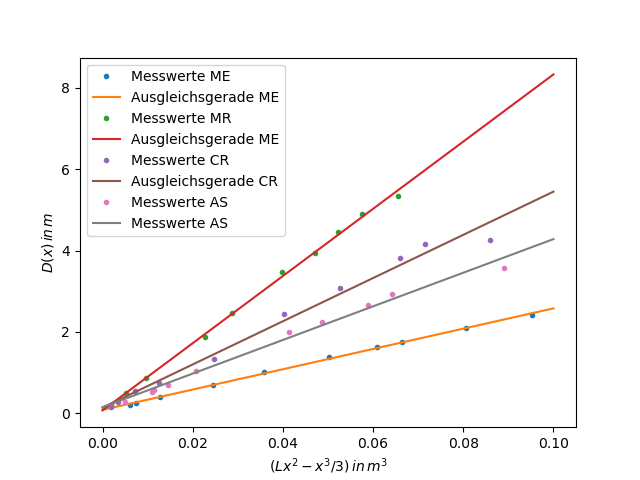
\includegraphics{Daten/AS1.png}
	\caption{Messdaten und Fit für das einseitige einhängen der Stangen.}
	\label{fig:einseitig}
\end{figure}

\noindent
Die Messwerte lassen sich nun in die \autoref{fig:einseitig} eintragen und Mithilfe einer Regressionsgerade der Form $$ D = a*x + b$$ ergibt sich

\begin{align*}
    \text{für cr}:& a = (53.1455 \pm 2.21684) \, \si{1\per\meter^2} ; \, b = (0.13443\pm 0.10422) \, \si{\meter}  \\
    \text{für mr}:& a = (82.6638 \pm 1.11642 ) \, \si{1\per\meter^2} ;\, b = (0.06684\pm 0.04410) \, \si{\meter}  \\
    \text{für ms}:& a = (24.9591 \pm 0.29885) \, \si{1\per\meter^2} ; \, b = (0.08105\pm 0.08105) \, \si{\meter}  \\
\text{und für as}:& a = (41.3532 \pm 1.54561) \, \si{1\per\meter^2} ;\,  b = (0.14570\pm 0.06994) \, \si{\meter} \, .\\
\end{align*} 

\noindent
Mithilfe der \autoref{eqn:deins} lässt sich der Zusammenhang
\begin{equation*}
    E = \frac{F_\text{G}}{2a_x\symbf{I}}.
\end{equation*}

\noindent
bestimmen, wobei $F_\text{G}= m \cdot g$ die Gewichtskraft mit $g = \SI{9.81}{\meter\per\second\squared}$ ist, sodass sich das Elastizitätsmodul berechnen lässt zu 
\begin{align*}
    \text{cr}:& E = (1.41 \pm 0.06  ) \cdot 10^{11} \, \si{\newton\per\meter²}\\
    \text{mr}:& E = (0.907 \pm 0.012) \cdot 10^{11} \, \si{\newton\per\meter²}\\
    \text{ms}:& E = (1.468 \pm 0.018) \cdot 10^{11} \, \si{\newton\per\meter²}\\
    \text{as}:& E = (0.783\pm 0.029 ) \cdot 10^{11} \, \si{\newton\per\meter²} \, .\\
\end{align*} 

Der statistische Fehler ergibt sich mit der Gaußschen Fehlerfortpflanzung zu: 

\begin{equation*}
\Delta E = \frac{\partial E}{\partial m_1}\cdot \Delta m_1 
= \frac{-F_\text{G}}{2\symbf{I}m²} \cdot \Delta m_1 ß, .
\end{equation*}

\subsection{Beidseitig eingehängt Stange}
Das vorgehen ist äquivalent zum Kapitel nur das diesmal die Stangen an zwei Stellen eingespannt werden in einem Abstand von $L = 55 \, \si{\centi\meter}$.
 Diesmal wird bei den Stangen folgende Massen bei der Länge $x$ eingehangen. Die Messergebnisse befinden sich in den folgenden Tabellen.
\begin{align*}
    \text{cr}:& m = 747.2 \, \si{\gram}; \,  x = 28 \, \si{\centi\meter} \\
    \text{mr}:& m = 1238.5 \, \si{\gram};\,  x = 27.5 \, \si{\centi\meter} \\
    \text{ms}:& m = 1238.5 \, \si{\gram};\,  x = 27.5 \, \si{\centi\meter} \\
    \text{as}:& m = 747.2 \, \si{\gram}; \,  x = 28 \, \si{\centi\meter}   \\
\end{align*}

\begin{table}
	\centering
	\caption{Messwerte zu der eckige Kupferstange, beidseitig eingehangen.} 
	\label{tab:vana} 
	\begin{tabular}{c c c}
	\toprule
	$\text{Seite des Gewichts} $&$x \, / \, \si{\centi\meter}$ & $D \, / \, \si{\micro\meter}$\\
	\midrule
    $\text{Links}$    &    35     &    315 \\
        &    40     &    265 \\
        &    45     &    180 \\
        &    47     &    141 \\
        &    50     &    105 \\
    $\text{Rechts}$    &    9       &    72 \\
        &    12      &   115 \\
        &    15      &   161 \\
        &    19      &   230 \\
        &    23      &   268 \\
\bottomrule
	\end{tabular}
\end{table}

\begin{table}
	\centering
	\caption{Messwerte zu der runden Messingstange, beidseitig eingehangen.} 
	\label{tab:vana} 
	\begin{tabular}{c c c}
	\toprule
	$\text{Seite des Gewichts} $&$x \, / \, \si{\centi\meter}$ & $D \, / \, \si{\micro\meter}$\\
	\midrule
    $\text{Links}$ & 33     &     570\\
    & 37     &     650\\
    & 40     &     575\\
    & 43     &     515\\
    & 46     &     500\\
    $\text{Rechts}$ & 5      &      35\\
    & 9      &     125\\
    & 13     &     220\\
    & 18     &     360\\
    & 23     &     472\\
\bottomrule
	\end{tabular}
\end{table}

\begin{table}
	\centering
	\caption{Messwerte zu der eckigen Messingstange, beidseitig eingehangen.} 
	\label{tab:vana} 
	\begin{tabular}{c c c}
	\toprule
	$\text{Seite des Gewichts} $&$x \, / \, \si{\centi\meter}$ & $D \, / \, \si{\micro\meter}$\\
	\midrule
    $\text{Links}$ & 49.65   &     37\\
    &47     &      72\\
    &45     &      81\\
    &40     &     112\\
    &35     &     139\\
    $\text{Rechts}$ & 9       &     40\\
    &11.3  &       57\\
    &15    &       78\\
    &19    &     99.5\\
    &21    &      112\\
\bottomrule
	\end{tabular}
\end{table}


\begin{table}
	\centering
	\caption{Messwerte zu der eckigen Aluminiumstange, beidseitig eingehangen.} 
	\label{tab:vana} 
	\begin{tabular}{c c c}
	\toprule
	$\text{Seite des Gewichts} $&$x \, / \, \si{\centi\meter}$ & $D \, / \, \si{\micro\meter}$\\
	\midrule
    $\text{Links}$  &45       &   88\\
                    &37.3     &  195\\
                    &51.05    &   60\\
                    &33.8     &  210\\
                    &40       &  179\\
    $\text{Rechts}$ &14       &   85\\
                    &13.7     &  100\\
                    &18.41    &  129\\
                    &18.4     &  131\\
                    &8.01     &   35\\
\bottomrule
	\end{tabular}
\end{table}

\noindent
Nun lassen sich die rechte und linke Seite unabhängig von einander in den \autoref{fig:rechts} und \autoref{fig:links} darstellen und wie schon zuvor mittels einer
Regressionsgeraden fitten. Im weiteren Verlauf der Auswertung wird jedoch nur die rechte Stabseite betrachtet, also die für die $ 0 \, \leq \, x \, \leq \, L/2$. 

\begin{figure}[H]
	\centering
	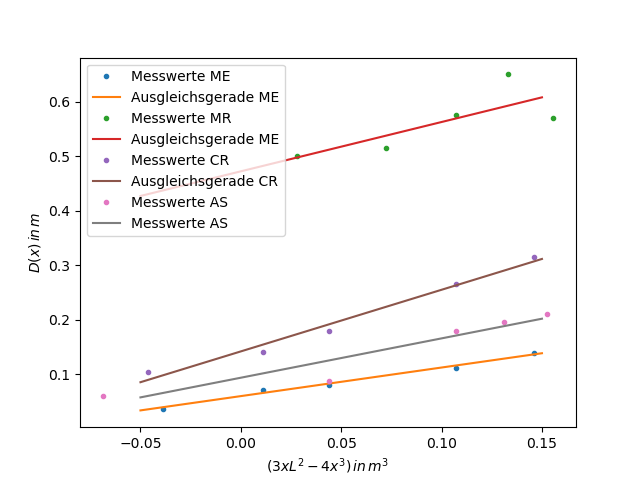
\includegraphics{Daten/AS2_r.png}
	\caption{Messdaten und Fit für das beidseitige einhängen der Stangen, rechts.}
	\label{fig:rechts}
\end{figure}

\begin{figure}[H]
	\centering
	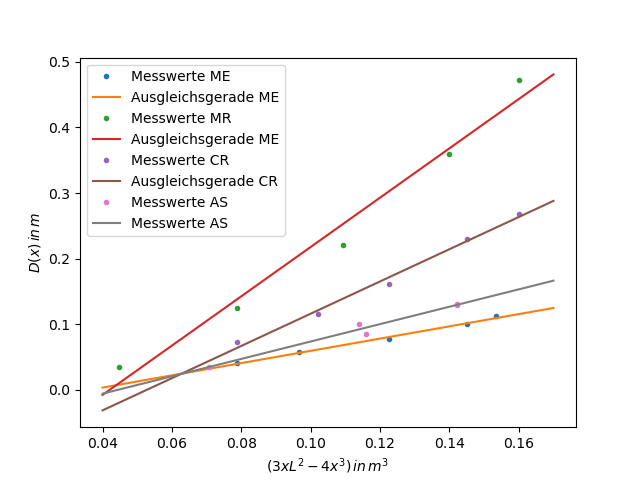
\includegraphics{Daten/AS2_l.png}
	\caption{Messdaten und Fit für das beidseitige einhängen der Stangen, links.}
	\label{fig:links}
\end{figure}

\noindent
Aus den Fitts folgt
\begin{align*}
    \text{für cr}:& a = (1.1304 \pm 0.09432) \, \si{1\per\meter^2} ; \, b = (0.1419 \pm 0.00811) \, \si{1\per\meter^2}  \\
    \text{für mr}:& a = (0.9044 \pm 0.43141) \, \si{1\per\meter^2} ; \, b = (0.4722 \pm 0.04703) \, \si{1\per\meter^2} \\
    \text{für ms}:& a = (0.5242 \pm 0.52424) \, \si{1\per\meter^2} ; \, b = (0.0599 \pm 0.00279) \, \si{1\per\meter^2}\\
\text{und für as}:& a = (0.7214 \pm 0.13761) \, \si{1\per\meter^2} ;\,  b = (0.0937 \pm 0.01487) \, \si{1\per\meter^2} \, .\\
\end{align*} 

\noindent
Mithilfe der \autoref{eqn:d1} lässt sich der Zusammenhang 
\begin{equation*}
    E = \frac{F_\text{G}}{48a_\text{x}\symbf{I}}
\end{equation*}

\noindent
feststellen. Damit folgt für das Elastizitätsmodul
\begin{align*}
    \text{cr}:& E = (2.75 \pm 0.23) \cdot 10^{11}   \, \si{\newton\per\meter²}\\
    \text{mr}:& E = (5.7 \pm 2.7) \cdot 10^{11} \, \si{\newton\per\meter²}\\
    \text{ms}:& E = (4.83 \pm 0.03) \cdot 10^{11} \, \si{\newton\per\meter²} \\
    \text{as}:& E = (2.5\pm 0.5) \cdot 10^{11} \, \si{\newton\per\meter²} \, .\\
\end{align*} 

